\documentclass{beamer}

\usepackage[utf8]{inputenc}
\usepackage{default}


\usepackage{multirow} %for aligning stuff in tables

\usepackage{bbding} %for the smiley face

\usepackage{calc} %calculate spacing \widthof

%tikz stuff
\usepackage{tikzsymbols}
\usepackage{tikz}
\usetikzlibrary{fit,arrows,positioning}

  % Keys to support piece-wise uncovering of elements in TikZ pictures:
  % \node[visible on=<2->](foo){Foo}
  % \node[visible on=<{2,4}>](bar){Bar}   % put braces around comma expressions
  %
  % Internally works by setting opacity=0 when invisible, which has the 
  % adavantage (compared to \node<2->(foo){Foo} that the node is always there, hence
  % always consumes space plus that coordinate (foo) is always available.
  %
  % The actual command that implements the invisibility can be overriden
  % by altering the style invisible. For instance \tikzsset{invisible/.style={opacity=0.2}}
  % would dim the "invisible" parts. Alternatively, the color might be set to white, if the
  % output driver does not support transparencies (e.g., PS) 
  %
  \tikzset{
    invisible/.style={opacity=0},
    visible on/.style={alt={#1{}{invisible}}},
    alt/.code args={<#1>#2#3}{%
      \alt<#1>{\pgfkeysalso{#2}}{\pgfkeysalso{#3}} % \pgfkeysalso doesn't change the path
    },
  }
  \tikzset{
    dimmed/.style={opacity=0.2},
    dimmed on/.style={alt={#1{dimmed}{}}},
    alt/.code args={<#1>#2#3}{%
      \alt<#1>{\pgfkeysalso{#2}}{\pgfkeysalso{#3}} % \pgfkeysalso doesn't change the path
    },
  }
\tikzset{
    %Define standard arrow tip
    >=stealth',
    %Define style for boxes
    peer/.style={
           rectangle,
           rounded corners,
           draw=black, thin,
           text width=3.5em,
           minimum height=2em,
           text centered},
    node/.style={
           rectangle,
           rounded corners,
           draw=black, 
           text width=4.5em,
           minimum height=2em,
           text centered,
           fill={rgb:black,1;white,3}},
    chunk/.style={
           rectangle,
           rounded corners,
           draw=black, 
           text width=2.5em,
           minimum height=1em,
           text centered,
           fill=block title bg},
    % Define arrow style
    point/.style={
           ->,
           thick,
           shorten <=2pt,
           shorten >=2pt,}
every node/.style={align=center}           
}

\newcommand{\wholeslide}[2][]{
\begin{frame}{#1}
% \transboxout<1>[duration=0.5]
\setbeamercolor{bgcolor}{fg=black,bg=white}
\begin{tikzpicture}[overlay, remember picture]
\node[anchor=center] at (current page.center) {
  \begin{beamercolorbox}[center]{bgcolor}
     #2
  \end{beamercolorbox}};
\end{tikzpicture}

\end{frame}
}

\newenvironment<>{varblock}[2][.9\textwidth]{%
  \setlength{\textwidth}{#1}
  \begin{actionenv}#3%
    \def\insertblocktitle{#2}%
    \par%
    \usebeamertemplate{block begin}}
  {\par%
    \usebeamertemplate{block end}%
  \end{actionenv}}

\newlength{\mywidth}
\newcommand{\blockslide}[3][]{
\settowidth{\mywidth}{#3}
\begin{frame}[c]{#1}
\begin{center}
\begin{minipage}{1.1\mywidth}
 \begin{varblock}[1.1\mywidth]{#2}
  #3
 \end{varblock}
\end{minipage}
\end{center}
\end{frame}
}

\mode<presentation>{
\usetheme{Warsaw}\usecolortheme{crane}
\setbeamertemplate{items}[square]
\setbeamertemplate{section in toc}[square]
\setbeamertemplate{subsection in toc}[square]
% \setbeamertemplate{subsection in toc}[subsections numbered]
\setbeamertemplate{subsubsection in toc}[square]
% \setbeamercolor{items}{fg=black,bg=yellow}
\usebeamercolor{block title}
\definecolor{block title bg}{named}{bg}
\setbeamercolor{item projected}{fg=black,bg=block title bg}
\setbeamercolor{itemize item}{fg=block title bg,bg=block title bg}
}







\title{Swarm}
\author{Viktor Tron and Aron Fischer}

\AtBeginSection[]
{
\begin{frame}<beamer>
\frametitle{Outline}
\tableofcontents[currentsection,sectionstyle=show/shaded,subsectionstyle=show/show/hide,subsubsectionstyle=show/show/show/hide]
\end{frame}
}

\begin{document}
 
\begin{frame}
 \titlepage
\end{frame}

\begin{frame}
 \tableofcontents[subsectionstyle=shaded/shaded,subsubsectionstyle=hide/hide]
\end{frame}


\section[Files and Chunks]{A (very quick) overview of data in swarm}



\subsection{Data in}
% \wholeslide{Data in: Saving data to the swarm.}
\blockslide{\textbf{Data in}}{Saving data to the swarm.}
\subsubsection{Chunking}
\wholeslide{1. Chunking: breaking up the data}

\begin{frame}[t]{\alt<5->{It's chunks all the way down...}{Chunks}}
% \begin{overlayarea}{⟨area width⟩}{⟨area height⟩}
%   ⟨environment contents⟩
% \end{overlayarea}
\begin{overlayarea}{\textwidth}{10cm}
Under the hood swarm does not deal in files but in \emph{chunks.}

\begin{itemize}
 \item<2-> All data is broken into pieces of size 4kB: ``chunks".
 \item<4-> Chunks are hashed and the hash is used as their ID/address.
 \item<5-> Chunk hashes are also packaged into 4kB chunks...
\end{itemize}

\begin{onlyenv}<1-2>
 \begin{center}
  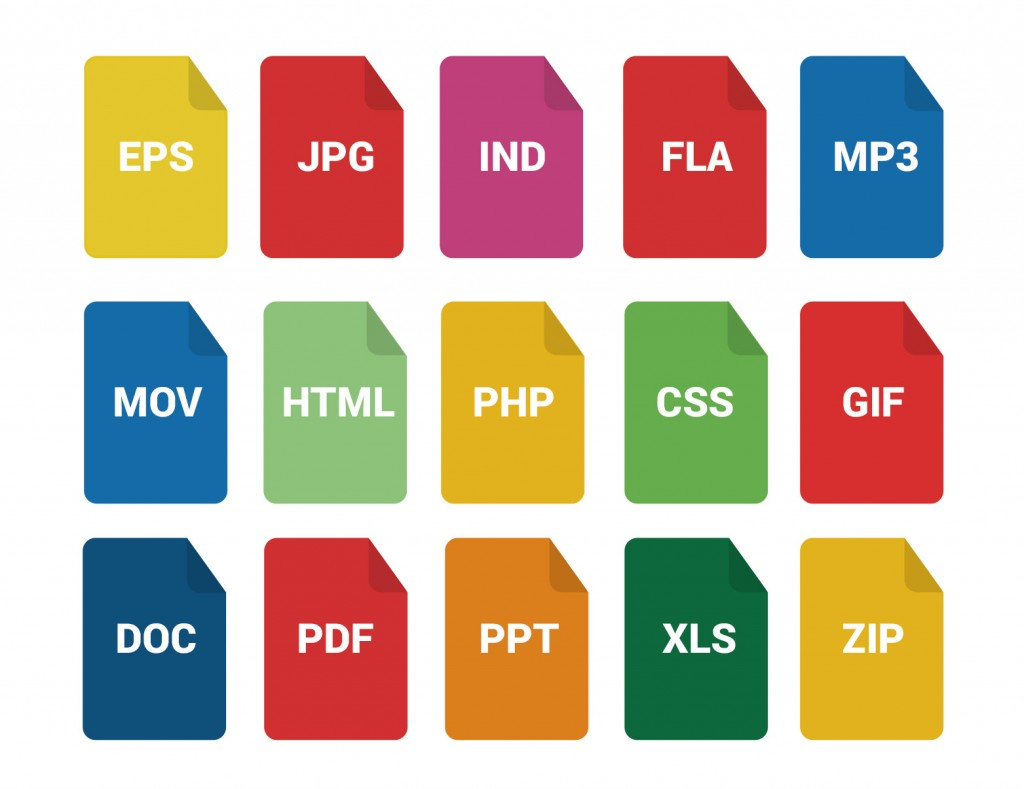
\includegraphics[width=0.4\textwidth]{files.jpg}
  \transdissolve<3>
 \end{center}
\end{onlyenv}

 \begin{center}
  \begin{tikzpicture}
   \node[chunk,visible on=<3>] at (0,0) (achunk){};
   \node[visible on=<3>] at (-1.8,0) (labeltext){A ``chunk:"};
   \node[chunk,visible on=<3->] at (-4,-3) (a){};
   \node[chunk,visible on=<3->] at (-2,-3) (b){};
   \node[chunk,visible on=<3->] at (0,-3) (c){};
   \node[chunk,visible on=<3->] at (2,-3) (d){};
   \node[chunk,visible on=<3->] at (4,-3) (e){};
   
   \node at (-4.2,-1.3) (dummy1) {};
   \node at (4.2,-1.7) (dummy2) {};
   \node[chunk,fit=(dummy1)(dummy2),visible on=<5>]{};
   
   \node[scale=0.8,draw,visible on=<4-5>] at (-4,-1.5) (ha){$h_1$}
     (a.north) edge[-,visible on=<4>] (ha.south);
   \node[scale=0.8,draw,visible on=<4-5>] at (-2,-1.5) (hb){$h_2$}
     (b.north) edge[-,visible on=<4>] (hb.south);
   \node[scale=0.8,draw,visible on=<4-5>] at (0,-1.5) (hc){$h_3$}
     (c.north) edge[-,visible on=<4>] (hc.south);
   \node[scale=0.8,draw,visible on=<4-5>] at (2,-1.5) (hd){$h_4$}
     (d.north) edge[-,visible on=<4>] (hd.south);
   \node[scale=0.8,draw,visible on=<4-5>] at (4,-1.5) (he){$h_5$}
     (e.north) edge[-,visible on=<4>] (he.south);
   
   \node[chunk,visible on=<6>] at (0,-1.5) {};
     \end{tikzpicture}

 \end{center}
\end{overlayarea}
\end{frame}

\subsubsection{Encoding}
\wholeslide{2. Encoding: Assembling the chunks into a merkle tree.}

\begin{frame}[t]{Everything is merkle-ised.}
When you want to save a document (or collection) to swarm, the swarm client
\begin{enumerate}
 \item<2-> Assembles all chunks into a merkle tree...
 \item<3-> ...including extra redundancy (``parity chunks").
 \item<4-> Returns a single \textbf{root hash} for the entire collection.
\end{enumerate}
\uncover<5->{\textbf{Note:} This means that you entire collection is accessible and retrievable from this single hash.}

\begin{center}
 \begin{onlyenv}<2>
  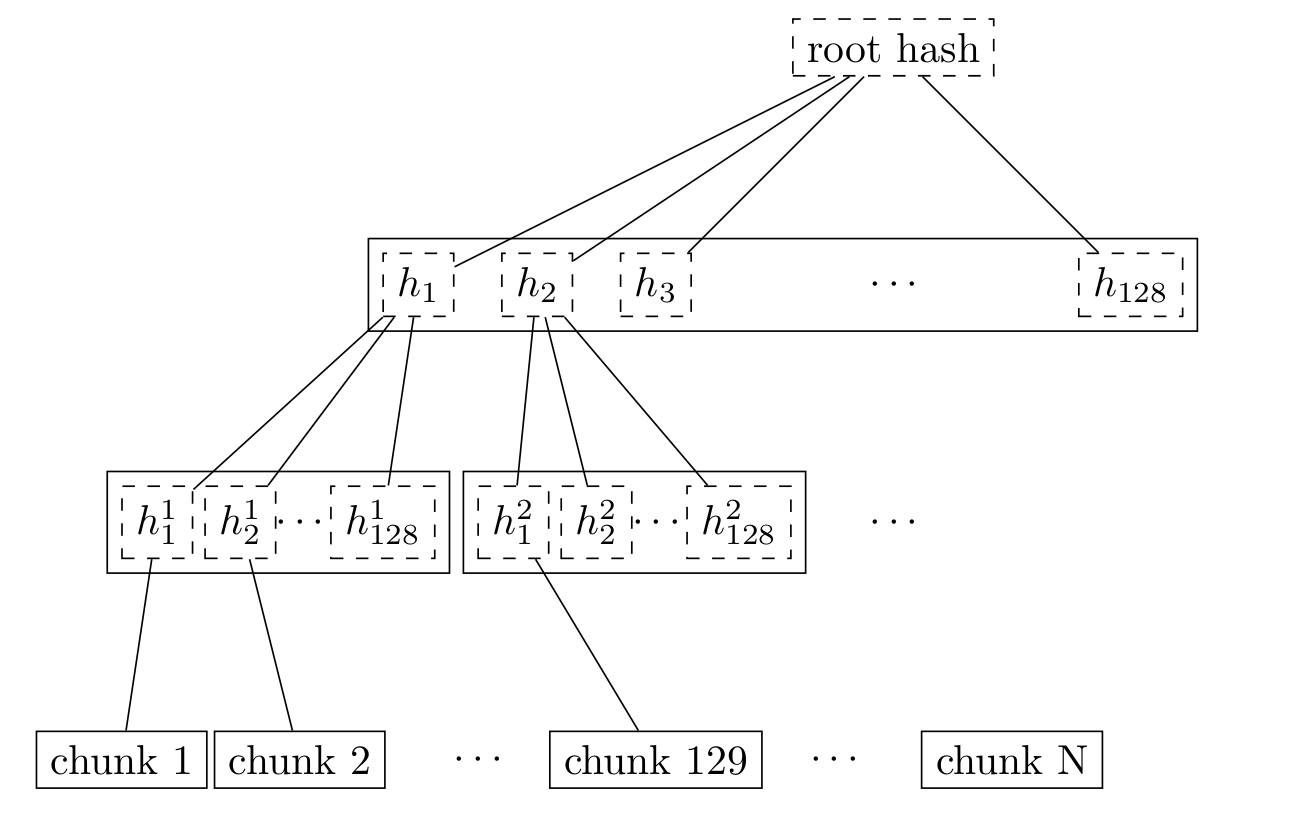
\includegraphics[width=0.5\textwidth]{chunk-tree.png}
 \end{onlyenv}
 \begin{onlyenv}<3>
  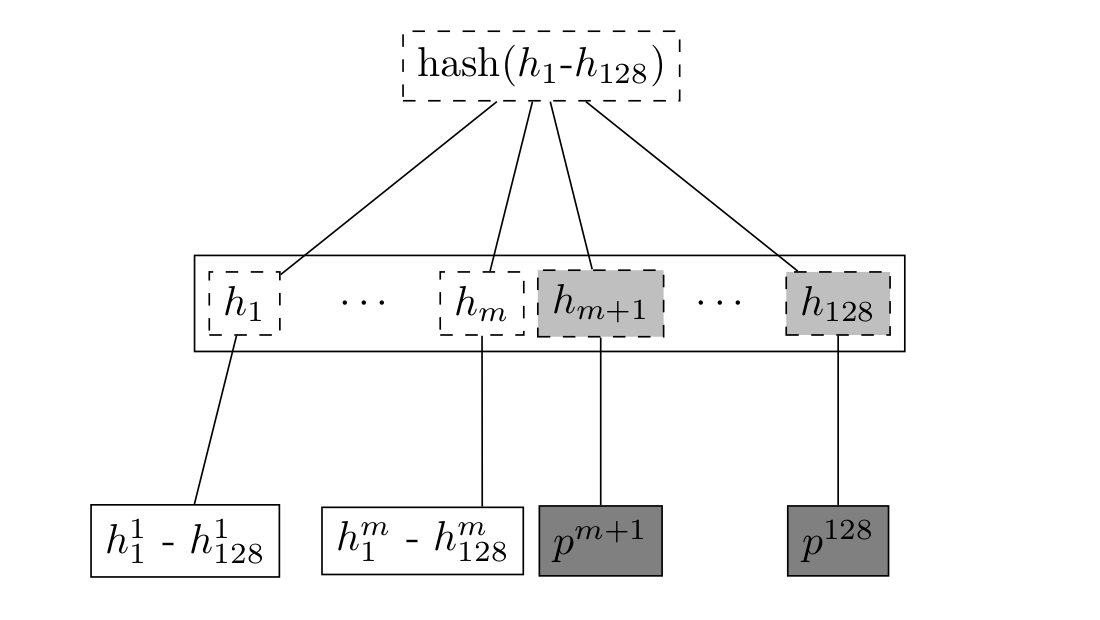
\includegraphics[width=0.5\textwidth]{erasure-coded-tree.png}
 \end{onlyenv}

\end{center}



\end{frame}



\subsubsection{Syncing}
\wholeslide{3. Syncing: getting the chunks to where they need to be.}

\begin{frame}{The syncing process.}
\begin{columns}[T]
\begin{column}{0.4\textwidth}
\small{The process of getting chunks to their storage destination is called \alert<1>{syncing}.}

\begin{itemize}
 \item<3-> \alt<5->{\tiny}{} Chunks are to be stored at\alt<4->{\alert<4>{ the node whose address is closest to}}{} the chunk ID. 
 \item<5-> \alt<7->{\tiny}{} Instead of directly connecting to that node and giving it the chunk in question, we pass the chunk along to one of our connected peers who is a little closer to the chunk ID than we are. \uncover<6->{``Syncing".}
 \item<7-> \alt<10->{\tiny}{} This peer will repeat the process, thus the data is passed on \uncover<8->{from node}\uncover<9->{ to node.}
 \item<10>[] %dummy. I needed this to get line spacing to work in the point above.
\end{itemize}
{  }\pause
\end{column}

\begin{column}{0.6\textwidth} 
\begin{tikzpicture}
 \node[scale=0.7]{
    \begin{tikzpicture}
	\node[invisible] at (0,-9) (dummy){};
	\node[invisible] at (5,-5) (dummy2){};
	\node[peer,visible on=<2->] at (-2,0) (owner){Owner};

	\node[visible on=<3->] (chunk) at (4,-5) {$\bullet$};
	\node[visible on=<3->] (chunklabel) at (5,-4) {chunk address} edge[point,->,visible on =<3->] (chunk);

	\node[peer,visible on=<5->] at (0.5,-0.5) (connectedpeer){peer}
	    (owner.east) edge[point, ->,visible on=<6->, bend left=15] 
		    node[above=2pt,visible on=<6->] {sync}
			    (connectedpeer.150);
			    
	\node[node,visible on=<7->] at (1,-2) (firstnode){some node}
		(connectedpeer.-70) edge[point,->,visible on=<7->,bend left=10] 
		    node[right of=2pt,visible on=<7->] {sync} 
			    (firstnode.north);

	\node[node,visible on=<8->] at (0.5,-4.5) (secondnode){other node}
		(firstnode.-70) edge[point,->,dashed,visible on=<8->,bend left=10] 
		    node[right of=2pt,visible on=<8->] {syncing...} 
			    (secondnode.70);

	\node[peer,visible on=<4->] at (4,-6) (closestnode){closest node}
		(secondnode.-110) edge[point,->,visible on=<9->,out=-110,in=180]
		    node[above=2pt,visible on=<9->] {sync}
			    (closestnode.west);
    \end{tikzpicture}
    };
\end{tikzpicture}
\end{column}
\end{columns}

\end{frame}

\wholeslide{ }

\subsection{Data out}

% \wholeslide{Data out: How to retrieve data stored in the swarm.}
\blockslide{\textbf{Data out}}{How to retrieve data stored in the swarm.}

\begin{frame}{Data Retrieval}
 When retrieving data from the swarm remember:
 \begin{itemize}
  \item<2-> All data is in chunks.
  \item<3-> All chunks are addressed by their hashes.
  \item<4-> Chunks are stored on nodes that are closest to the chunk hash.
 \end{itemize}
\end{frame}

\begin{frame}
 
\begin{tikzpicture}
\node[peer,visible on=<1->] at (12,0) (retriever){Retriever};
\node[visible on=<13>,scale=2] at (12,-1) {\Smiley};

\node[visible on=<2->] (chunk) at (4,-5) {$\bullet$};
\node[visible on=<2->] (chunklabel) at (3,-4) {chunk address} edge[point,->,visible on =<2->] (chunk);

\node[peer,visible on=<4-12>, dimmed on=<13->] at (8.5,-0.5) (connectedpeer){peer}
    (retriever.-150) edge[point, ->,visible on=<5>,dimmed on=<6-12>,  bend left=15] 
	    node[below=2pt,visible on=<5>, dimmed on=<6-12>] {request}
		    (connectedpeer.-10);
		    
\node[node,visible on=<6-11>, dimmed on=<12->] at (6,-2) (firstnode){some node}
	(connectedpeer.-70) edge[point,->,visible on=<6>, dimmed on=<7-11>,bend left=30] 
	    node[right of=2pt,visible on=<6>, dimmed on=<7-11>] {request} 
		    (firstnode.east);

\node[node,visible on=<7-10>, dimmed on=<11->] at (7.5,-4.5) (secondnode){other node}
	(firstnode.-70) edge[point,->,dashed,visible on=<7>, dimmed on=<8-10>,bend left=10] 
	    node[right of=2pt,visible on=<7>, dimmed on=<8-10>] {requests...} 
		    (secondnode.120);

\node[peer,visible on=<3-9>, dimmed on=<10->] at (4,-6) (closestnode){closest node}
	(secondnode.-110) edge[point,->,visible on=<8>, dimmed on=<9>,out=-110,in=0]
	    node[right of=2pt,visible on=<8>, dimmed on=<9>] {request}
		    (closestnode.east)
	(closestnode) edge[thick,point,->,visible on=<9>] node[above=2pt,visible on=<9>]{deliver} (secondnode)
	(secondnode.north west) edge[thick, point,->,visible on=<10>, dashed] node[left of=2pt,visible on=<10>]{deliveries} (firstnode.-120)
	(firstnode.55) edge[thick,point,->,visible on=<11>] node[left of=2pt,visible on=<11>]{deliver} (connectedpeer.-150)
	(connectedpeer) edge[thick,point,->,visible on=<12>] node[above=2pt,visible on=<12>]{deliver} (retriever)
	;
\end{tikzpicture}
\end{frame}

\wholeslide{ }

\section[Incentives]{Incentive Structure}
\subsection{A (simplified) history of WWW Incentivisation}
\subsubsection{Web 1.0}
\wholeslide{\Large{Incentive structure of Web 1.0}}
\begin{frame}{Incentive structure of Web 1.0}
  Back in the day...\\
  \begin{enumerate}
    \item<2-> Start up a webserver (or rent one)
    \item<3-> Upload some content (FTP)
  \end{enumerate}
  \begin{center}
    \begin{tabular}{ccc}
      \multicolumn{1}{l}{\uncover<4->{\textbf{Content is unpopular}}}	  & \multicolumn{2}{l}{\uncover<6->{\textbf{Content becomes popular}}}\\
      \multicolumn{1}{l}{\uncover<5->{$\bullet$ Pay running costs}}	  & \multicolumn{2}{l}{\uncover<7->{$\bullet$ Bandwidth costs skyrocket}}\\
      \multirow{2}{*}{\uncover<5->{
\includegraphics[scale=0.2]{smallcoinpile.png}}} & \multicolumn{2}{l}{\uncover<8->{$\bullet$ Server crashes and goes offline.}}\\
      & \uncover<7->{$\qquad$
\includegraphics[scale=0.2]{bigcoinpile.png}} & \uncover<8->{
\includegraphics[scale=0.2]{servercrash.jpg}}
    \end{tabular}
  \end{center}
 \begin{flushright}
  \uncover<9>{...but at least you owned your content.}
  \end{flushright}
\end{frame}

\subsubsection{Web 2.0}
\wholeslide{\Large{Incentive structure of Web 2.0}}
\begin{frame}{Web 2.0}
 Today\alt<1>{...}{ we just upload our content to ``the cloud".}\\[5pt]
 \uncover<3->{The cloud is:}\\
 \begin{itemize}
  \item<3-> Cheap \uncover<4->{or even \alt<5->{``free"}{free}} 
  \item<6-> Scalable
  \item<7-> Reliable
 \end{itemize}
 \uncover<8->{\Large{\alert{But...}}\\}
 \begin{itemize}
  \item<9-> Content is \alert<9>{owned by the service providers}.
  \item<10-> All users are \alert<10>{tracked and spied on}; providers profit off the data.
  \item<11-> Centralised control: \alert<11>{surveillance and censorship}.
 \end{itemize}
\pause
\end{frame}


\subsubsection{Peer-to-peer (p2p)}
\blockslide{}{\Large{What about p2p?}}
\begin{frame}{Properties of the bittorrent network}
 \only<1>{Let's talk about }Bittorrent\\
 \uncover<2->{\textbf{Pros:}}
 \begin{itemize}
  \item<2-> Content is distributed among peers.
  \item<3-> Distribution scales automatically.
  \item<4-> Hashing ensures data integrity.
  \item<5-> No central point of failure (no servers).
 \end{itemize}
 \uncover<6->{\textbf{Cons:}}
 \begin{itemize}
  \item<6-> Downloads start slowly (high latency).
  \item<7-> No incentive to provide content: ``seeding".
 \end{itemize}
\end{frame}

\wholeslide{\transboxout}

\subsection{Incentivisation in Swarm}
\blockslide{}{Incentivisation in Swarm }
\wholeslide{
\begin{flushleft}
We want all the benefits of p2p \uncover<2->{...\\while using ethereum to pay and get paid}\uncover<3->{, aligning everyone's individual incentives with those of the network.} 
\end{flushleft}
}

\subsubsection{Introduction}
\begin{frame}{Swarm Incentive System}
\begin{columns}[t]
  \column{.5\textwidth}
    \begin{block}<2->{Bandwidth}
     \uncover<3->{$\bullet$ Account for all bandwidth used (p2p).\\}
     \uncover<4->{$\bullet$ Compensate nodes based on provided bandwidth.}
    \end{block}
  \column{.5\textwidth}
    \begin{block}<2->{Storage}
      \uncover<5->{$\bullet$ Allow for long term storage of data.}\\
      \uncover<6->{$\bullet$ Provide proper compensation for nodes storing the data.}
    \end{block}
\end{columns}
\end{frame}

\subsubsection{Bandwidth}
\wholeslide[Dealing with Bandwidth]{\Large{Bandwidth}}
\begin{frame}{Dealing with Bandwidth}
 Bandwidth accounting \alt<2>{\alert{has to be}}{is} peer-to-peer.\\
 \begin{center}
  \begin{tikzpicture}
   \node[peer,visible on=<3->] at (-3,0) (node1) {Me};
   \node[peer,visible on=<4->] at (3,0) (node2) {Peer}
   (node1.50) edge[point,->,dashed,visible on=<5->,bend right=30,out=50,in=130] node[below=10pt,visible on=<7->,scale=0.8] (sup){\# of chunks supplied} (node2.130)
   (node2.-130) edge[point,->,dashed,visible on=<6->,bend left=30,in=130,out=50] node[above=10pt,visible on=<9->,scale=0.8]{\# of chunks received} (node1.-50)
   ;
   \node[visible on=<8->,below of=sup]{\Large{-}};
  \end{tikzpicture}
 \end{center}
 \uncover<10->{Note: Only involves Request/Deliver, not syncing.}
\end{frame}

\wholeslide{SWAP: \textbf{Sw}arm \textbf{A}ccounting \textbf{P}rotocol}

\begin{frame}{SWAP: Swarm Accounting Protocol}
\textbf{The Swarm Accounting Protocol}
\begin{itemize}
 \item<2-> Keeps track of chunks provided/received (per peer)
 \item<3-> Can trade chunk-for-payment\alt<3>{}{ and chunk-for-chunk}
\end{itemize}
\uncover<5->{\textbf{Payments}}
\uncover<6->{use the swarm chequebook smart contract.}
\uncover<7->{Cheques are \textit{cumulative} and are sent off-chain. Only the last cheque needs to be cashed. This saves transaction costs and blockchain bloat.\\[5pt]}
\uncover<8->{\textbf{\alert{Soon:} Raiden payment-channel integration!}}
\end{frame}

\begin{frame}{SWAP: Swarm Accounting Protocol}
\Large{Big picture:}
\begin{itemize}
 \item<2-> If you download a lot of content, you \textbf<2>{pay your peers} for providing it.
 \item<3-> If you host popular content, you will \textbf<3>{earn fees from your peers} for making the content available.
 \item<4-> The Swarm is \textbf<4>{auto-scaling}! \uncover<5->{\\\small{-interplay of routing protocol and per-chunk payment between peers means that popular content will be widely distributed thereby increasing available bandwidth while decreasing latency}}
\end{itemize}
\end{frame}
\begin{frame}
 \begin{tikzpicture}
\node[peer,visible on=<1->] at (12,0) (retriever){};

\node[visible on=<1->] (chunk) at (4,-5) {$\bullet$};
\node[visible on=<1->] (chunklabel) at (3,-4) {chunk address} edge[point,->,visible on =<1->] (chunk);

\node[node,visible on=<2->,] at (8.5,-0.5) (connectedpeer){}
    (retriever.-150) edge[point, ->,visible on=<4-8>,  bend left=15] 
	    node[below=2pt,visible on=<4>] {request}
		    (connectedpeer.-10);
		    
\node[node,visible on=<2->] at (6,-2) (firstnode){}
	(connectedpeer.-70) edge[point,->,visible on=<4-7>,bend left=30] 
	    node[right of=2pt,visible on=<4>] {request} 
		    (firstnode.east);

\node[node,visible on=<2->] at (7.5,-4.5) (secondnode){}
	(firstnode.-70) edge[point,->,dashed,visible on=<4-6>,bend left=10] 
	    node[right of=2pt,visible on=<4>] {requests...} 
		    (secondnode.120);

\node[peer,visible on=<2->] at (4,-6) (closestnode){}
	(secondnode.-110) edge[point,->,visible on=<4-5>,out=-110,in=0]
	    node[right of=2pt,visible on=<4>] {request}
		    (closestnode.east)
	(closestnode) edge[thick,point,->,visible on=<5>] (secondnode)
	(secondnode.north west) edge[thick, point,->,visible on=<6>, dashed] (firstnode.-120)
	(firstnode.55) edge[thick,point,->,visible on=<7>] (connectedpeer.-150)
	(connectedpeer) edge[thick,point,->,visible on=<8>] (retriever)
	;
\node[chunk, scale=0.6,visible on=<3->, below=5pt of closestnode.70] {}; 
\node[chunk, scale=0.6,visible on=<5->, below=5pt of secondnode.70] {};
\node[chunk, scale=0.6,visible on=<6->, below=5pt of firstnode.70] {};
\node[chunk, scale=0.6,visible on=<7->, below=5pt of connectedpeer.70] {};
\node[chunk, scale=0.6,visible on=<8->, below=5pt of retriever.70] {};

\node[peer, visible on=<10->] at (12,-6) (newguy){};
\node[node, visible on=<11->] at (11,-4) (newnode){}
    (newguy) edge[point,->,visible on=<12-15>,dashed,bend left=20] (newnode)
    (newnode) edge[point,->,visible on=<13-14>,bend left=20] (secondnode)
    ;

\node[chunk, scale=0.6,visible on=<14->, below=5pt of newnode.70] {}
    (secondnode) edge[thick,point,->,visible on=<14>] (newnode);
\node[chunk, scale=0.6,visible on=<15->, below=5pt of newguy.70] {}
    (newnode) edge[thick,point,->,visible on=<15>] (newguy);

\node[visible on=<16>,scale=4] at (3,-1) {\Smiley};

\end{tikzpicture}
\end{frame}


\wholeslide{ }

\subsubsection{Storage}
\blockslide[Dealing with storage]{}{Storage}
\begin{frame}{Dealing with storage}
\begin{center}
 \only<1>{\Large{Alas... we don't have the time}}
%  \only<2>{\includegraphics[width=0.8\textwidth]{nottoday1.jpg}}
%  \only<3>{\includegraphics[width=0.8\textwidth]{nottoday.jpg}}
\end{center}
\end{frame}

\begin{frame}
 Ok. Very quickly:\\
 \uncover<2->{The \textbf{SWEAR} contract takes security deposits.\\}
 \uncover<3->{Swear registered nodes can sell promises of long term data storage.\\}
 \uncover<4->{The \textbf{SWINDLE} contract enforces these promises with proof-of-custody litigation engine.}
\end{frame}


\section[Status and Roadmap]{Status and Roadmap}
\subsection[Status]{Status: Where are we at?}
\subsubsection{Swarm clients}
\begin{frame}{Status: Swarm Clients}
Currently there is a swarm enabled geth client only (github, swarm branch $\rightarrow$ develop).\\
\uncover<2->{Soon swarm will be a standalone daemon.}
\end{frame}

\subsubsection{Testnet}
\begin{frame}{Status: Swarm Testnet}
There is a testnet up and running.\\
\texttt{http://web3.download} is a direct http proxy to a swarm node\\
There is an ENS (name service) running on the swarm. For example you can access the page named 'swarm' at:\\
	      \texttt{http://web3.download/bzz:/swarm/}
\end{frame}

\subsubsection{Incentives}
% \wholeslide[Status: Incentives]{
% \Large{
%   \textbf{SWAP}\alt<1>{\textbf{?}}{ \CheckmarkBold$\quad$}
%   \uncover<3->{\textbf{SWEAR}\alt<3>{\textbf{?}}{ \Checkmark}$\quad$}
%   \uncover<5->{\textbf{SWINDLE}\alt<5>{\textbf{?}}{ \XSolidBrush}}
%   }
%   \uncover<6>{   }
% }


% \begin{frame}
% \begin{tikzpicture}
% 
% \node at (0,0) (topleft){};
% \node[scale=0.5] at (1,-1) (fuse){
%   \begin{tikzpicture}
%       \node at (0,-5) (dummy1){d1};
%       \node at (2,0) (dummy2){d2};
%       \node[draw,rounded corners,fit=(dummy1)(dummy2)] (thenode) at (0,0){
%       };
%     \node[scale=0.5,below = 2pt of thenode.100] {
\includegraphics[width=1cm]{fuse.jpg}};
%     \node[scale=0.7,text width=5em] at (0,-1) {hello fuse text};
%   \end{tikzpicture}
% };
% \node at (20,-10) (bottomright) {};
% \end{tikzpicture}
% 
% \end{frame}


\begin{frame}{Features and Implementation}
% \begin{overlayarea}{⟨area width⟩}{⟨area height⟩}
%   ⟨environment contents⟩
% \end{overlayarea}
\begin{overlayarea}{\textwidth}{10cm}
\setbeamercovered{transparent}% Dim out "inactive" elements
\begin{columns}[t]
  \column{0.5\textwidth}
    \begin{block}<1->{Feature}
      \begin{enumerate}
       \item<2,7> \textbf<2>{Efficacy \& Efficiency} 
       \item<3,7> \textbf<3>{Reliability}
       \item<4,7> \textbf<4>{Data Integrity}
       \item<5,7> \textbf<5>{User Authentication}
       \item<6-7> \textbf<6>{Attribution}
      \end{enumerate}
    \end{block}
    \begin{block}<2-6>{Why?}
      \only<2>{So that all content is accessible, popular content has low latency (comp. Web2)}
      \only<3>{So that stored content does not get lost}
      \only<4>{So that we aren't given bad data.}
      \only<5>{So that only people with proper authorisation can access content}
      \only<6>{So that content producers are recognised}
    \end{block}
  \column{0.5\textwidth}
    \begin{block}<2-6>{How?}
      \only<2>{
	  SWAP incentive structure: popular content is readily available\\
	  Payment-channel integration (Raiden): fast and cheap
	  }
      \only<3>{
      \begin{itemize}
       \item Redundant storage
       \item Built-in erasure coding
       \item Proof-of-custody based insurance
       \item Automatic scan-and-repair
      \end{itemize}
      }
      \only<4>{
      \begin{itemize}
       \item Everything is stored in Merkle trees
       \item Merkle proof compatible file `manifests'
       \item Chunk traversal follows Merkle-proof logic
      \end{itemize}
      }
      \only<5>{Data is encrypted and signed. Identity is managed on user side.}
      \only<6>{ENS + smart contracts}
      \only<7>{
\includegraphics[width=0.4\textwidth]{swarmlogo.png} Swarm!}
    \end{block}
%     \begin{block}<4->
%      
%     \end{block}
\end{columns}
\end{overlayarea}
\end{frame}

% \begin{frame}
% 
% %  \begin{block}
% \tiny
% \begin{tabular}{llll}
% 
% security feature & remedy/guarantees & technologies components used & what is at stake\\
% %
% operational reliability. 
%   & to sure content is always ready. popular content lower latencies. delay should be conparable to web 2 
%     & bandwidth incentives 
%       & swap, payment channels, raiden\\
% %
% accessibility 
%   & that content is reliably stored should never delete 
%     & poc, redundancy, scan and repair, storage insurance
%       & smash crash, payment channels. conditional escrow\\
% %       
% content authentication = data integrity 
%   & multi layer hierarchical merkleisation
%     & merkle proof of manifest form, swarm chunker traversal for chunks and smash proofs for chunk internal 
%       & \\
% %
% authentication for identity 
%   & Make sure only those authorized can enter entries to public services 
%     & public key cryptography digital signatures 
%       & \\
% %
% authenticity attribution 
%   & have ways to prove origination, and links spread 
%     & measure the time and efficiency of your search 
%       & ens authors and book formats
%  
% \end{tabular}
% 
%   
%   
% %  \end{block}
% 
% \end{frame}

\subsection{Overview: Architecture}
\begin{frame}
\begin{overlayarea}{\textwidth}{10cm}
\begin{tikzpicture}
\node[scale=0.8] at (current page.center) {
\begin{tikzpicture}

 \node[draw,rounded corners] at (4,4) (goapi) {
\includegraphics[width=2cm]{golang.png} API};
 
 \node[draw,rounded corners] at (0,0) (ipc) {JSON IPC};
 \node[draw,rounded corners] at (4,0) (proxy) {http-
\includegraphics[width=1cm]{proxy.jpg}-proxy};
 \node[draw,rounded corners] at (8,0) (fuse) {fuse 
\includegraphics[width=1cm]{fuse.jpg}};
 
 \node[draw,rounded corners] at (2,-4) (cli) {CLI 
\includegraphics[width=1cm]{cli.png}};
 \node[draw,rounded corners] at (6,-4) (web3js) {web3.js};
 
 \node {}
 (cli) edge[point,->] (ipc)
 (web3js) edge[point,->] (ipc)
 (cli) edge[point,->] (proxy)
 (web3js) edge[point,->] (proxy)
 (cli) edge[point,->] (fuse)
 (web3js) edge[point,->] (fuse)
 (ipc) edge[point,->] (goapi)
 (proxy) edge[point,->] (goapi)
 (fuse) edge[point,->] (goapi)
 ;
\end{tikzpicture}
};
\end{tikzpicture}
\end{overlayarea}
\end{frame}


\begin{frame}{Network Layer}
\begin{overlayarea}{\textwidth}{10cm}
\begin{center}

\begin{tikzpicture}
\node[scale=1.2] at (current page.center){
\begin{tikzpicture}
\node[draw,rounded corners] at (0,0) (pss) {PSS};
\node[draw,rounded corners] at (-2,-2) (hive) {HIVE};
\node[draw,rounded corners] at (2,-2) (bzz) {BZZ};
\node[draw,rounded corners] at (0,-4) (devp2p) {DevP2P};
\node {}
(pss) edge[point,->] (bzz)
(pss) edge[point,->] (hive)
(bzz) edge[point,->] (devp2p)
(hive) edge[point,->] (devp2p)
;
\end{tikzpicture}
};
\end{tikzpicture}
 
\end{center}

\end{overlayarea}

\end{frame}

\begin{frame}[c]{}
\begin{overlayarea}{\textwidth}{10cm}
\begin{center}
\begin{tikzpicture}
\node[scale=1.2] at (current page.center){
\begin{tikzpicture}
\node[draw,rounded corners] at (0,0) (pss) {PSS};
\node[draw,rounded corners] at (3,0) (bzz) {BZZ}
 (pss) edge[->] (bzz);
\node[draw,rounded corners] at (3,2) (sync) {Sync}
  (sync) edge[->] (bzz);
\node[draw,rounded corners] at (0,-2) (raiden) {Raiden}
  (raiden) edge[->] (pss);
\node[draw,rounded corners] at (3,-2) (swap) {SWAP}
  (swap) edge[->] (bzz);
\node[draw,rounded corners] at (-2,0) (swindle) {SWINDLE}
  (swindle) edge[->] (pss);
\node[draw,rounded corners] at (0,2) (sr) {
      \begin{tabular}{c}
      Scan \&\\
      Repair
      \end{tabular}
      }
  (sr) edge[->] (pss);
\node[draw,rounded corners] at (5.5,0) (req) {
    \begin{tabular}{c}
    Request\\
    Handler
    \end{tabular}
    }
  (req) edge[->] (bzz);

\end{tikzpicture}
};
\end{tikzpicture}
\end{center}

\end{overlayarea}
\end{frame}


\subsection[Roadmap]{Roadmap: What's next for Swarm?}
\begin{frame}
What else?
 \begin{itemize}
  \item<1-> Payment-channel integration into swarm (Raiden)
  \item<2-> Swarm-routing integration into Raiden
  \item<3-> Streaming Video -- project swatch to stream devcon over swarm
  \item<4-> Stable testnet and scalability testing (azure cloud)
  \item<5-> Dropbox and archiver
  \item<5-> ...and so much more.
  
 \end{itemize}

 
\end{frame}

\subsubsection{Scalability}
\wholeslide{ }
% \wholeslide[Payment Channels]{Payment Channels for SWAP}
% \begin{frame}{Payment Channels}
%  placeholder -- Raiden to swarm.
% \end{frame}
% 
% \wholeslide[State Channels]{State Channels for SWEAR and SWINDLE}
% \begin{frame}{State Channels}
%  placeholder -- the swindle judge contract.
% \end{frame}

\subsubsection{Streaming Media}
\wholeslide{ }
% \wholeslide[SWatch this Video]{Video chat and real-time communication}
% \begin{frame}{Project SWatch}
%  placeholder -- swatch
% \end{frame}
% 
% \wholeslide[Music]{Music with automatic industry payments}
% \begin{frame}{Music}
%  placeholder -- music and payment splits.
% \end{frame}

 
\end{document}
